\documentclass[12pt,a4paper]{article}
\usepackage{fontspec}
\defaultfontfeatures{Ligatures=TeX,Scale=MatchLowercase}
\IfFontExistsTF{Alice-Regular}{
  \setmainfont{Alice-Regular}[
      BoldFont = Alice-Regular,
      ItalicFont = Alice-Regular,
      BoldItalicFont = Alice-Regular,
      BoldFeatures = {FakeBold=1.6},
      ItalicFeatures = {FakeSlant=0.2},
      BoldItalicFeatures = {FakeBold=1.6,FakeSlant=0.2}
  ]
}{
  \setmainfont{Noto Serif}
}
\IfFontExistsTF{Noto Sans}{\setsansfont{Noto Sans}}{}
\usepackage{polyglossia}
\setmainlanguage{russian}
\usepackage[a4paper,left=20mm,right=20mm,top=20mm,bottom=20mm]{geometry}
\usepackage{graphicx}
\usepackage{amsmath,amssymb,amsthm}
\usepackage{booktabs,longtable,tabularx,array,float,multirow}
\usepackage{tikz}
\usepackage[europeanresistors]{circuitikz}
\usepackage{pgfplots}
\usepackage{xcolor}
\usepackage{caption}
\usepackage{fancyhdr}
\usepackage{enumitem}
\usepackage{tabularx}
\pgfplotsset{compat=1.18}
\pagestyle{fancy}
\fancyhf{}
\renewcommand{\headrulewidth}{0.4pt}
\renewcommand{\footrulewidth}{0.4pt}
\fancyfoot[C]{\thepage}
\newcolumntype{C}{>{\centering\arraybackslash}X}
\renewcommand{\arraystretch}{1.25}

\newcommand{\TitlePage}[2]{
\title{
	МИНОБРНАУКИ РОССИИ

	федеральное государственное автономное образовательное учреждение

	высшего образования

	«Национальный исследовательский университет

	«Московский институт электронной техники»
	\vspace{2em}
}
\author{}
\date{}
\maketitle
\thispagestyle{fancy}
\begin{center}
\Large Отчёт по лабораторной работе №#1\\
по дисциплине «Электротехника»\\
«#2»
\end{center}
\begin{center}
\Large Вариант 2
\end{center}
\vspace{12em}
\begin{table}[H]
\noindent
\begin{tabular*}{\textwidth}{@{\extracolsep{\fill}} p{0.48\textwidth} p{0.52\textwidth}}
Студент & Анисимов А.\,С., ЭН-$25$ \\
[0.5em] Руководитель & Самохин Д.\,В.
\end{tabular*}
\end{table}
\cfoot{Москва 2026}
\pagebreak
\fancyhead[L]{#2}
\fancyhead[R]{Электротехника}
}

\begin{document}
\TitlePage{4}{Исследование переходных процессов в цепях первого порядка}

\section*{Цель работы}
Исследовать переходные процессы в RL- и RC-цепях первого порядка при воздействии прямоугольных импульсов и обосновать используемые расчётные формулы через эквивалентное сопротивление схемы.

\section*{Исходные данные}
\textbf{RL-цепь:}
\[
E=48\,\text{В},\quad R_1=1.6\,\text{к}\Omega,\quad R_2=12\,\text{к}\Omega,\quad R_4=3\,\text{к}\Omega,\quad R_3=0.01\,\Omega,\quad L=40\,\text{мГн}.
\]

\textbf{RC-цепь:}
\[
E=10\,\text{В},\quad R_1=1.5\,\text{к}\Omega,\quad R_2=2\,\text{к}\Omega,\quad R_4=1\,\Omega,\quad R_3=0.01\,\Omega,\quad C=0.1\,\mu\text{Ф}.
\]

Так как частота импульсов в схемах методички существенно меньше обратной постоянной времени, к началу паузы ток в RL-цепи и напряжение на конденсаторе в RC-цепи практически достигают установившихся значений. Поэтому расчёт первых $0$, $5$ и $10\,\mu s$ удобно вести по экспоненциальным законам включения и отключения.

\section*{1. RL-цепь}
\subsection*{1.1. Схема замещения и аргументация выбора метода}
Узел с источником и сопротивлениями $R_1$, $R_2$ заменяем эквивалентным генератором Тевенина. Это удобно, потому что после такой замены индуктивность оказывается в обычной последовательной RL-цепи, для которой переходный процесс описывается одним дифференциальным уравнением первого порядка.

\begin{figure}[H]
\centering
\begin{circuitikz}
\draw
(0,0) to[american voltage source,l=$E_{\text{th}}$] (0,3)
      to[R,l=$R_{\text{th}}$] (3,3)
      to[R,l=$R_4+R_3$] (6,3)
      to[L,l=$L$] (6,0)
      -- (0,0);
\draw[->] (2.5,3.35) -- (3.5,3.35) node[midway,above] {$i_L(t)$};
\end{circuitikz}
\caption{Эквивалентная RL-схема после замены источника и делителя по Тевенину.}
\end{figure}

Эквивалентные параметры:
\[
R_{\text{th}}=R_1\parallel R_2=\frac{R_1R_2}{R_1+R_2}
=\frac{1.6\cdot 12}{1.6+12}\,\text{к}\Omega
\approx 1411.765\,\Omega,
\]
\[
E_{\text{th}}=E\frac{R_2}{R_1+R_2}
=48\cdot \frac{12}{1.6+12}
\approx 42.353\,\text{В}.
\]

Полное сопротивление ветви:
\[
R_\Sigma = R_{\text{th}}+R_4+R_3
\approx 4411.775\,\Omega.
\]

Постоянная времени:
\[
\tau_{RL}=\frac L{R_\Sigma}
=\frac{0.04}{4411.775}
\approx 9.067\,\mu\text{с}.
\]

Установившийся ток во время импульса:
\[
I_\infty=\frac{E_{\text{th}}}{R_\Sigma}
=\frac{42.353}{4411.775}
\approx 9.600\,\text{мА}.
\]

\subsection*{1.2. Законы изменения тока и напряжения}
При включении:
\[
i_L(t)=I_\infty\left(1-e^{-t/\tau_{RL}}\right),
\qquad
u_L(t)=E_{\text{th}}e^{-t/\tau_{RL}}.
\]

При отключении:
\[
i_L(t)=I_\infty e^{-t/\tau_{RL}},
\qquad
u_L(t)=-E_{\text{th}}e^{-t/\tau_{RL}}.
\]

Знак напряжения меняется, потому что после отключения индуктивность поддерживает прежнее направление тока и сама становится источником энергии.

\subsection*{1.3. Таблица значений для RL-цепи}
\begin{center}
\begin{tabularx}{\textwidth}{|C|C|C|C|}
\hline
Режим & $t$, $\mu s$ & $I_L(t)$, мА & $U_L(t)$, В \\
\hline
Импульс & 0 & 0.000 & 42.353 \\
\hline
Импульс & 5 & 4.069 & 24.400 \\
\hline
Импульс & 10 & 6.414 & 14.057 \\
\hline
Пауза & 0 & 9.600 & -42.353 \\
\hline
Пауза & 5 & 5.531 & -24.400 \\
\hline
Пауза & 10 & 3.186 & -14.057 \\
\hline
\end{tabularx}
\end{center}

\begin{figure}[H]
\centering
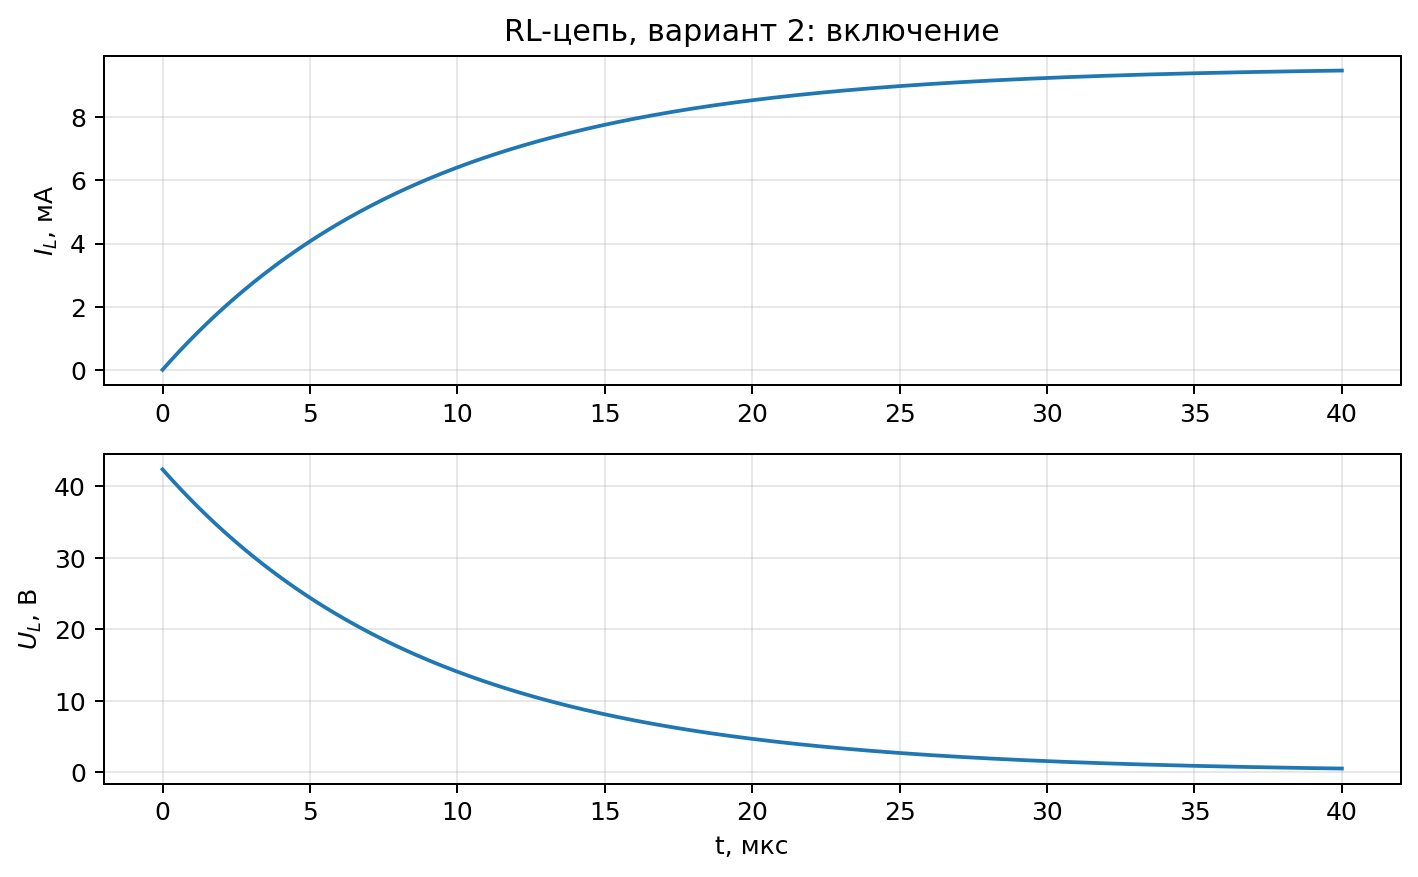
\includegraphics[width=0.82\textwidth]{img/lab4_rl_on.png}

\vspace{0.5em}
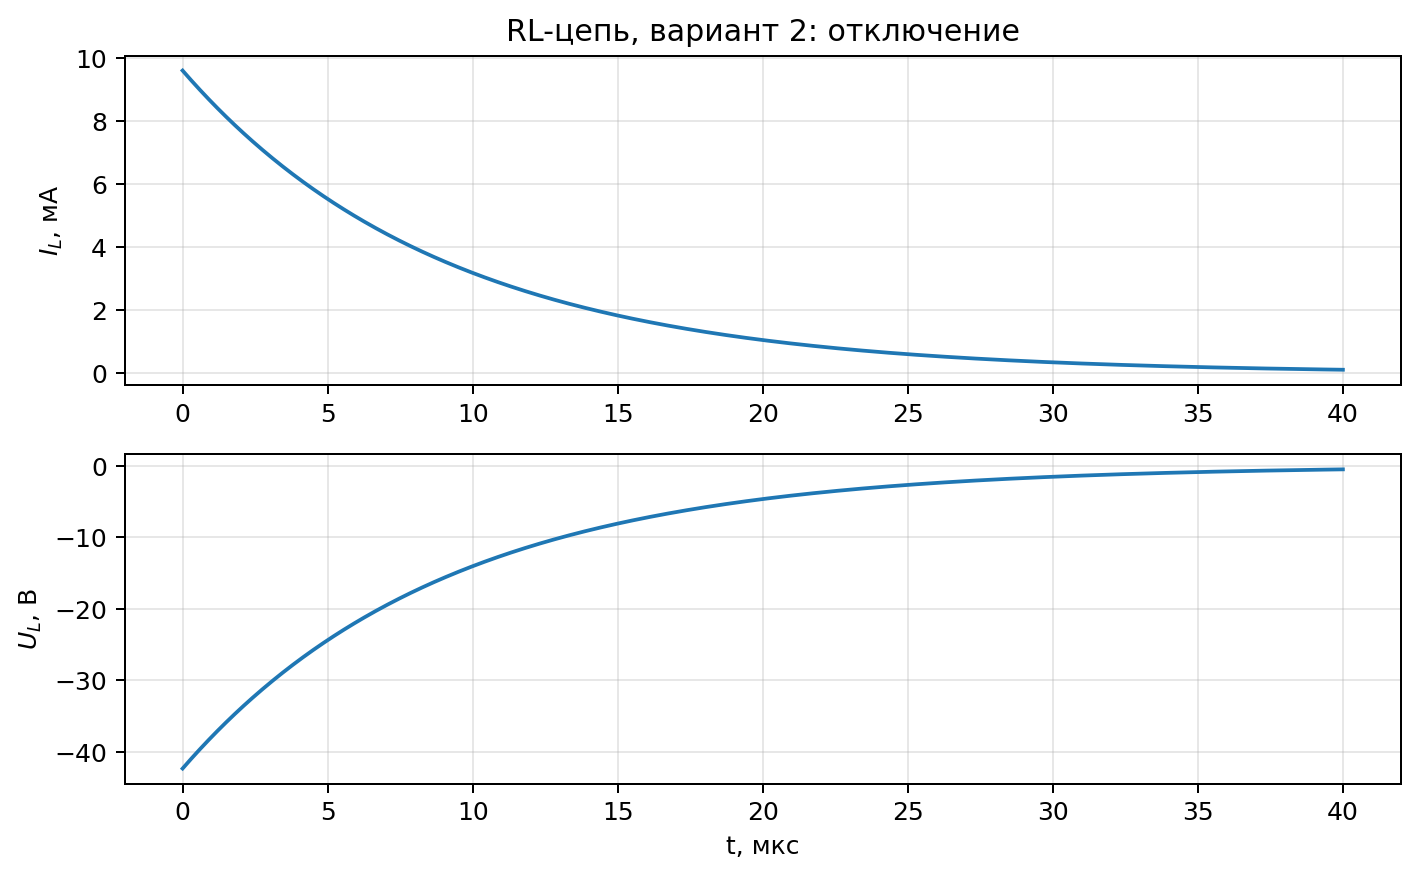
\includegraphics[width=0.82\textwidth]{img/lab4_rl_off.png}
\caption{Переходные процессы в RL-цепи: включение и отключение.}
\end{figure}

\section*{2. RC-цепь}
\subsection*{2.1. Схема замещения и аргументация выбора метода}
Для RC-цепи тот же приём с эквивалентом Тевенина делает схему одноконтурной. Это позволяет сразу записать постоянную времени как произведение ёмкости на сопротивление, ``видимое'' конденсатором.

\begin{figure}[H]
\centering
\begin{circuitikz}
\draw
(0,0) to[american voltage source,l=$E_{\text{th}}$] (0,3)
      to[R,l=$R_{\text{th}}+R_4+R_3$] (4,3)
      to[C,l=$C$] (4,0)
      -- (0,0);
\draw[->] (1.0,3.8) -- (3.0,3.8) node[midway,above] {$i_C(t)$};
\end{circuitikz}
\caption{Эквивалентная RC-схема после замены источника и делителя по Тевенину.}
\end{figure}

Эквивалентное сопротивление источника:
\[
R_{\text{th}}=R_1\parallel R_2=\frac{1.5\cdot 2}{1.5+2}\,\text{к}\Omega
\approx 857.143\,\Omega.
\]
Эквивалентная ЭДС:
\[
E_{\text{th}}=E\frac{R_2}{R_1+R_2}
=10\cdot \frac{2}{1.5+2}
\approx 5.714\,\text{В}.
\]
Полное сопротивление, видимое конденсатором:
\[
R_\Sigma = R_{\text{th}}+R_4+R_3 \approx 858.153\,\Omega.
\]
Постоянная времени:
\[
\tau_{RC} = R_\Sigma C
= 858.153\cdot 0.1\cdot 10^{-6}
\approx 85.815\,\mu\text{с}.
\]

Начальный ток зарядки:
\[
I_0=\frac{E_{\text{th}}}{R_\Sigma}
=\frac{5.714}{858.153}
\approx 6.659\,\text{мА}.
\]

\subsection*{2.2. Законы изменения тока и напряжения}
При зарядке:
\[
u_C(t)=E_{\text{th}}\left(1-e^{-t/\tau_{RC}}\right),
\qquad
i_C(t)=I_0e^{-t/\tau_{RC}}.
\]

При разрядке:
\[
u_C(t)=E_{\text{th}}e^{-t/\tau_{RC}},
\qquad
i_C(t)=-I_0e^{-t/\tau_{RC}}.
\]

Минус в выражении для тока при паузе указывает на изменение его направления относительно режима зарядки.

\subsection*{2.3. Таблица значений для RC-цепи}
\begin{center}
\begin{tabularx}{\textwidth}{|C|C|C|C|}
\hline
Режим & $t$, $\mu s$ & $I_C(t)$, мА & $U_C(t)$, В \\
\hline
Импульс & 0 & 6.659 & 0.000 \\
\hline
Импульс & 5 & 6.282 & 0.323 \\
\hline
Импульс & 10 & 5.926 & 0.629 \\
\hline
Пауза & 0 & -6.659 & 5.714 \\
\hline
Пауза & 5 & -6.282 & 5.391 \\
\hline
Пауза & 10 & -5.926 & 5.086 \\
\hline
\end{tabularx}
\end{center}

\begin{figure}[H]
\centering
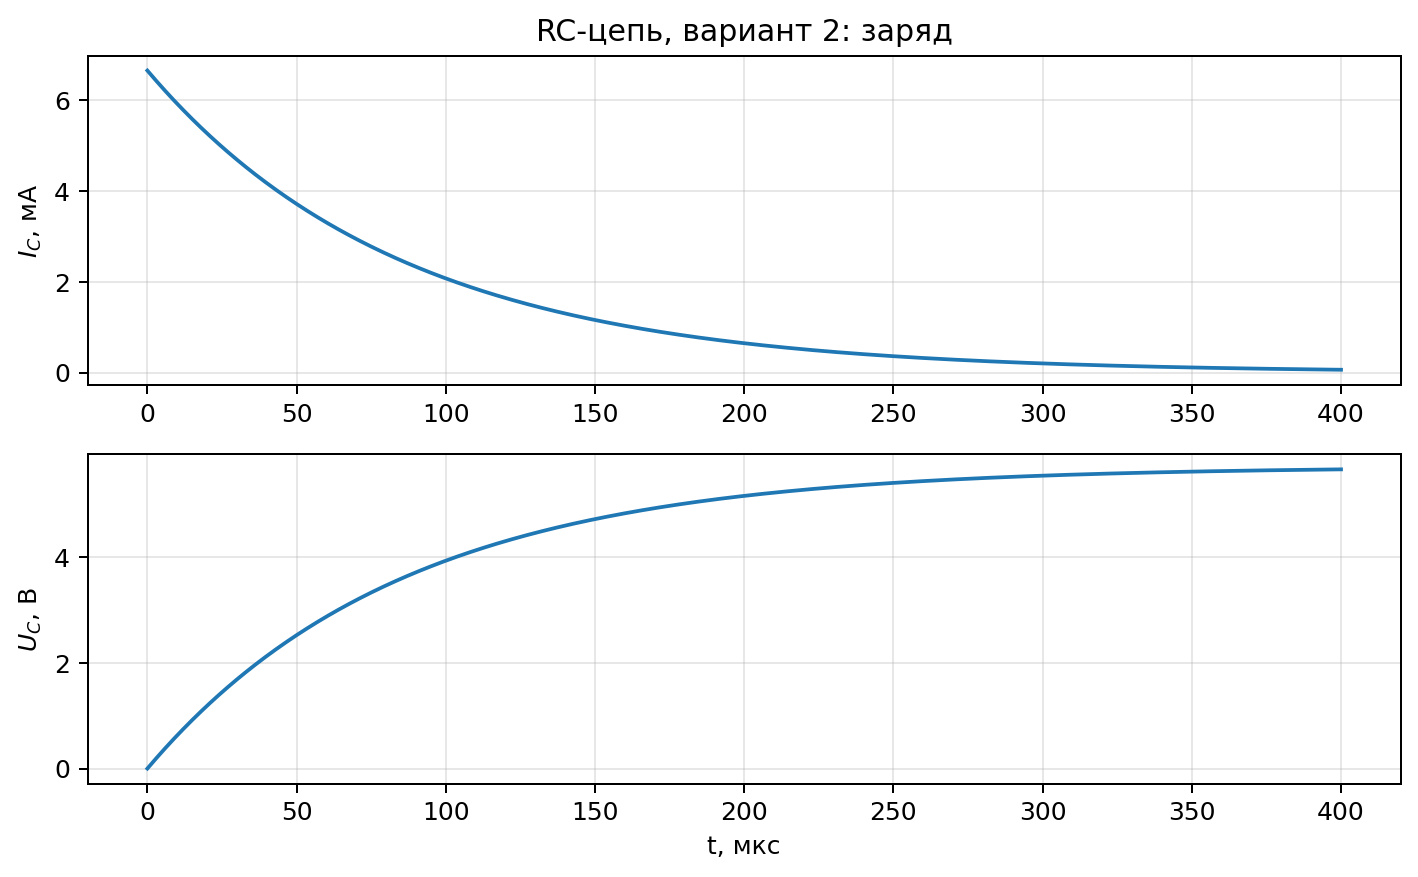
\includegraphics[width=0.82\textwidth]{img/lab4_rc_on.png}

\vspace{0.5em}
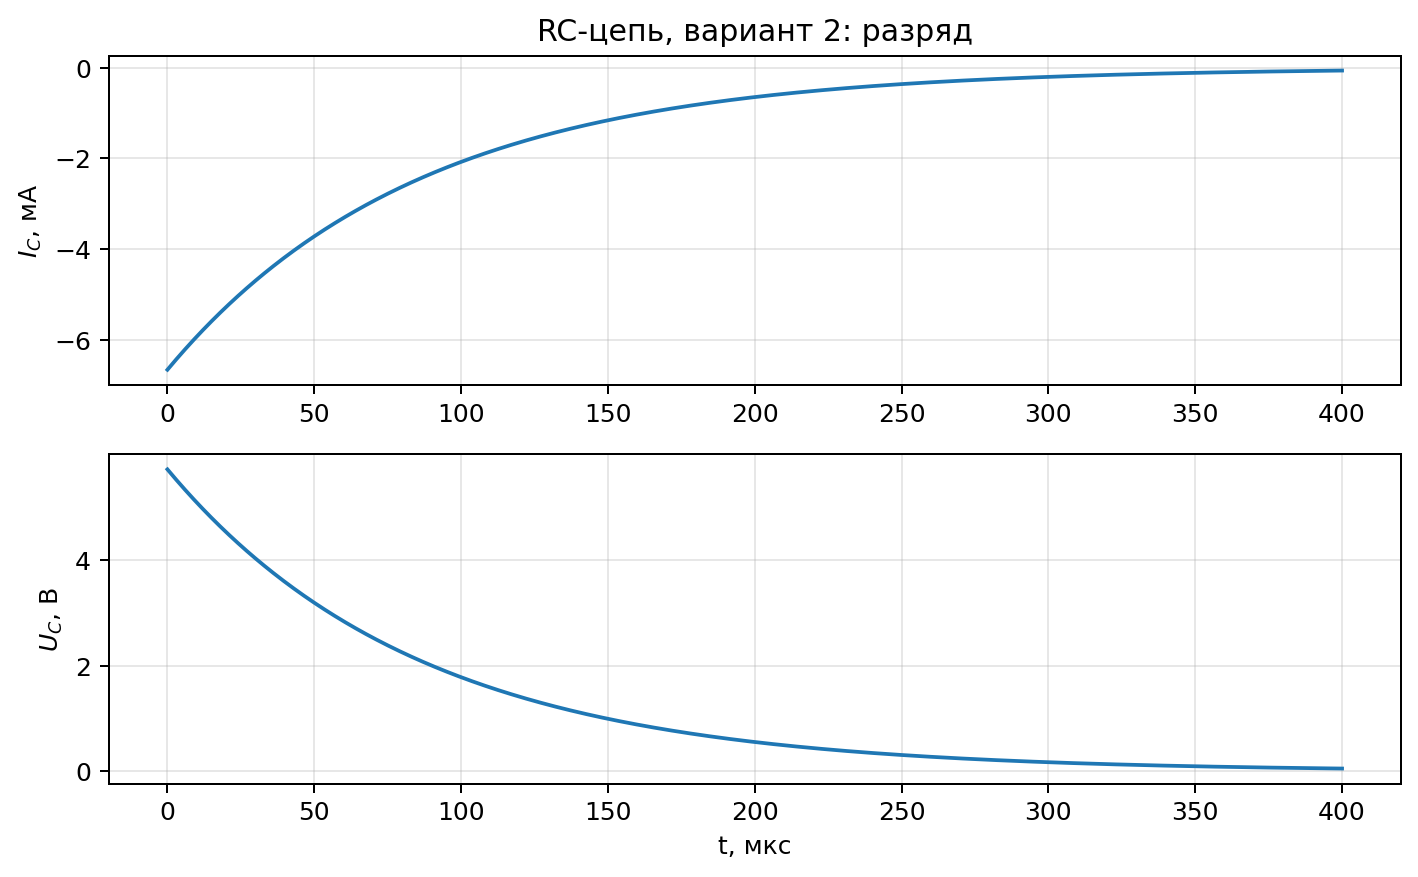
\includegraphics[width=0.82\textwidth]{img/lab4_rc_off.png}
\caption{Переходные процессы в RC-цепи: заряд и разряд.}
\end{figure}

\section*{Вывод}
Расчёт переходных процессов выполнен через эквивалентные параметры Тевенина, что позволило 
свести исходные схемы к простым RL- и RC-цепям первого порядка. Найдены постоянные времени 
$\tau_{RL}\approx 9.07\,\mu\text{с}$ и $\tau_{RC}\approx 85.82\,\mu\text{с}$, рассчитаны 
значения токов и напряжений в моменты $0$, $5$ и $10\,\mu s$ для импульса и паузы. 
Полученные графики подтверждают классические экспоненциальные законы: ток в индуктивности 
не меняется скачком, а напряжение на конденсаторе непрерывно.

\end{document}
